% 图 72.1 —— 由 `checks/emit_hand.py` 自动拼出（probe 精测 + prims2 图元分解）
%%
% ⚠ 这是**稿子不是成品**：跑 `checks/checkhand.py 72.1` 看指标 + 看叠合图。
%%
%% ⚠ 待核：
%   · 本图 probe 报出阴影族 2 个 —— **本脚本不生成阴影**（要照原书手写）；prims2 的 strokes 里可能含阴影线，核对时留意别画重
%   · 可疑字形 1 项（空心圈 ⊙ 常被认成字母 o）—— 见文件末
%%
\documentclass[12pt]{standalone}
\usepackage{fontspec}
\setsansfont{Arial}
\newfontfamily\mfallback{DejaVu Sans}
\usepackage{tikz}
\begin{document}
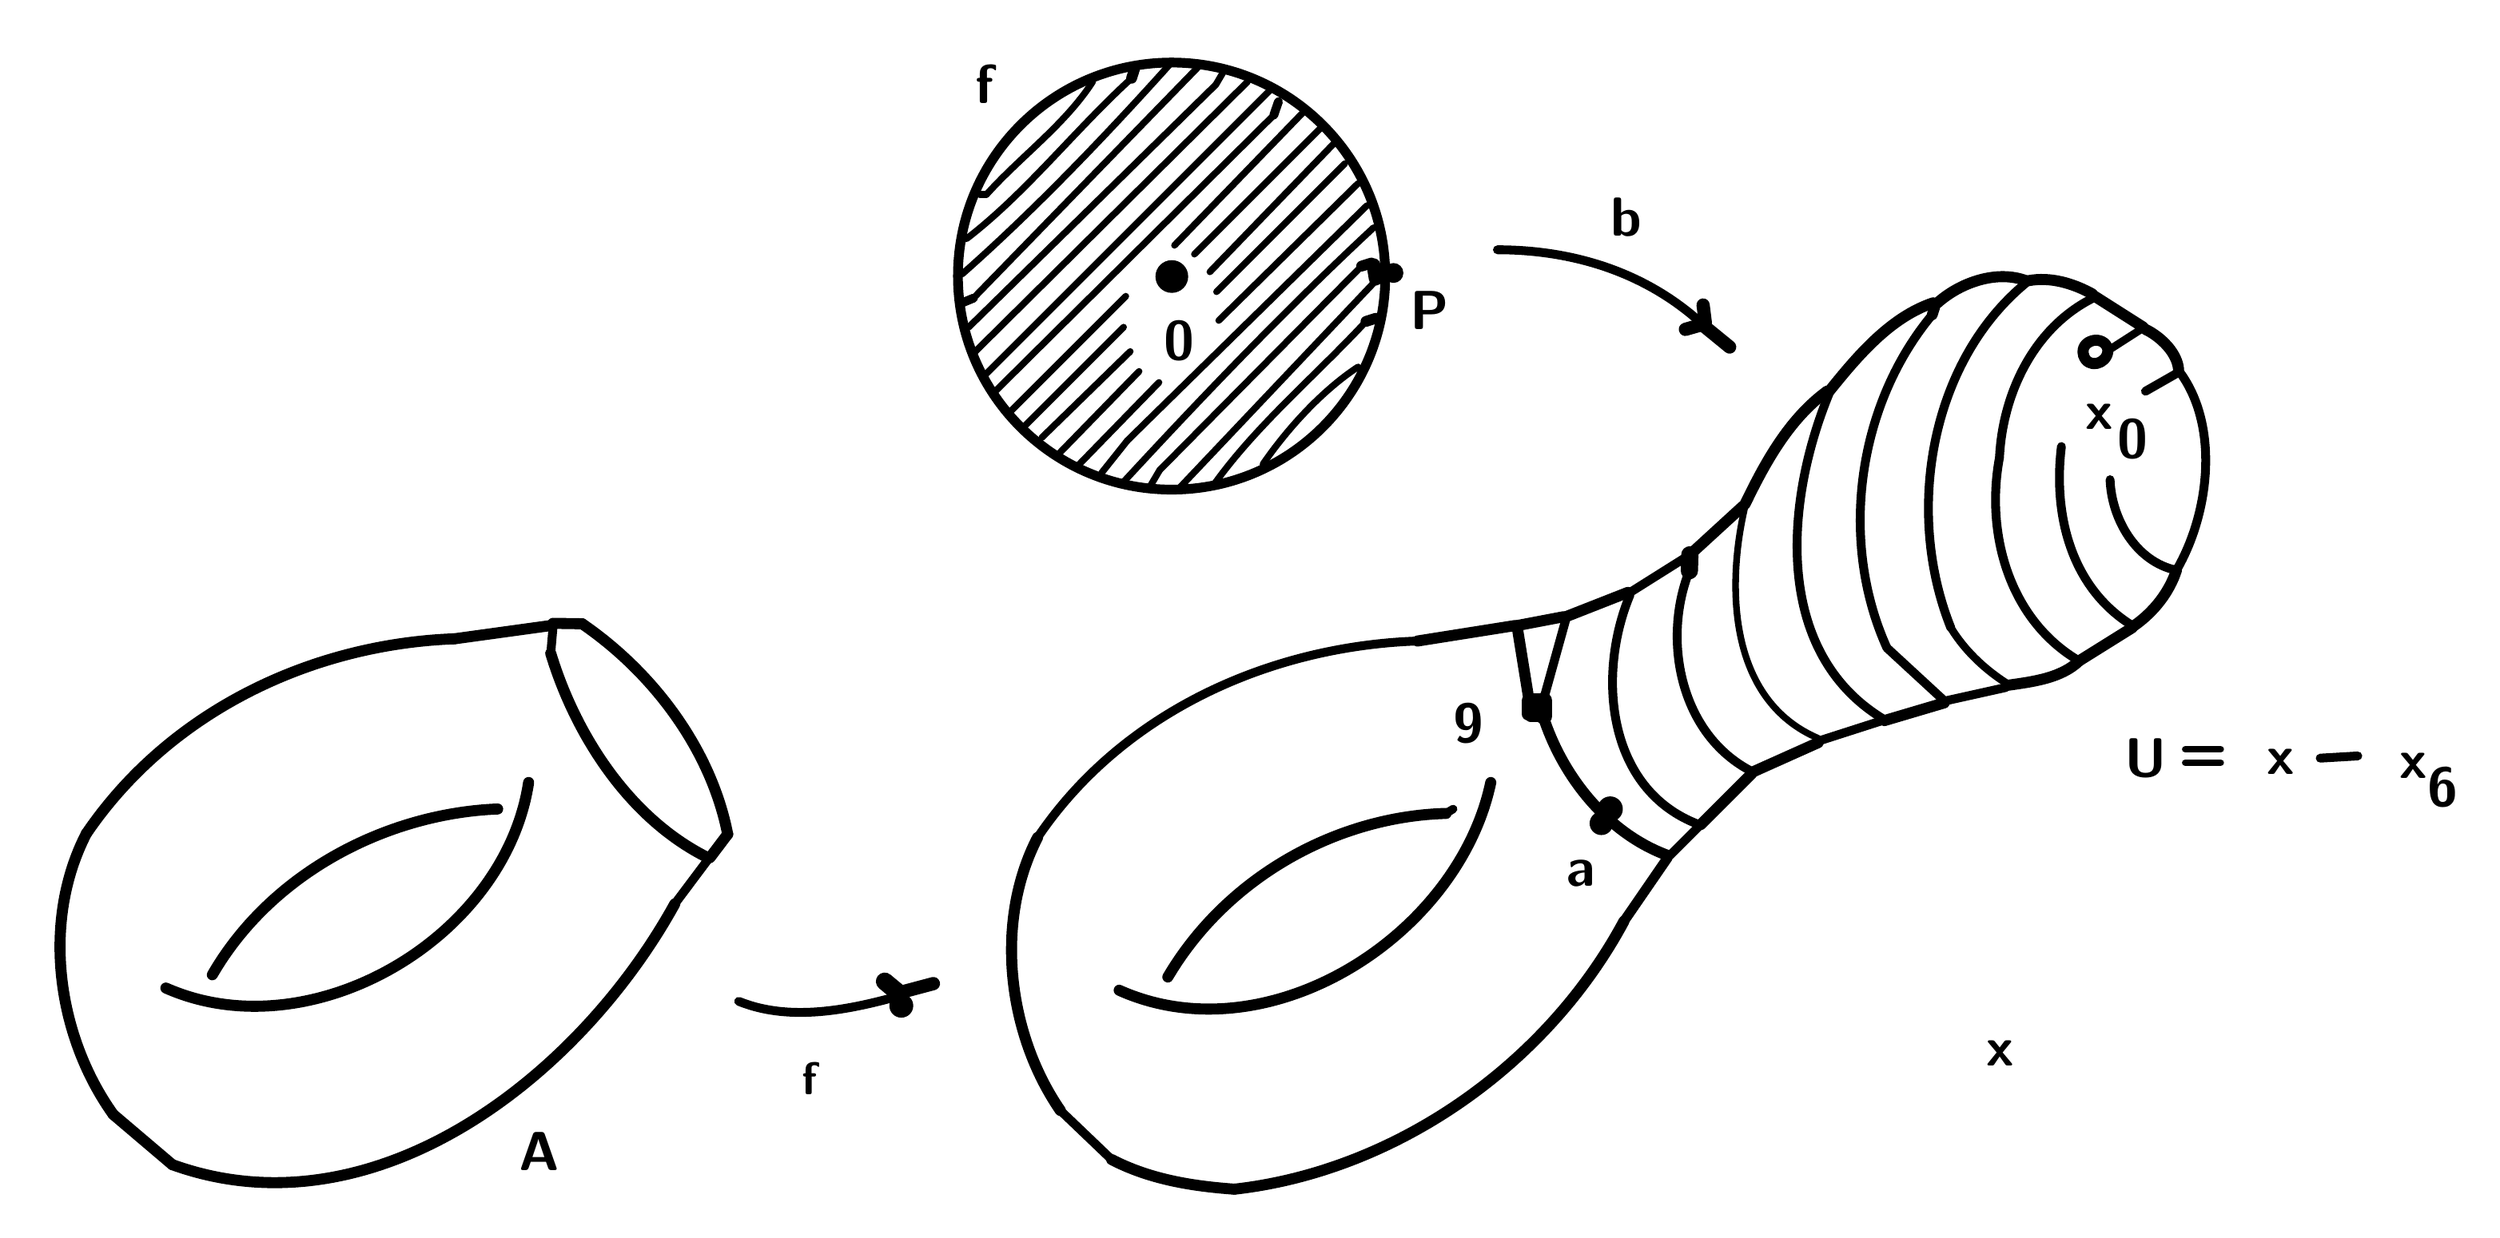
\begin{tikzpicture}[x=1pt, y=-1pt, line width=4.4pt, line cap=round, line join=round]

  %% ════ 填充区（prims2 的 fills）════

  %% ════ 直线段（prims2 的 strokes）════
  \draw[line width=3.0pt] (453.0,183.0) -- (498.0,138.0);
  \draw[line width=3.0pt] (540.0,122.0) -- (598.0,64.0);
  \draw[line width=6.0pt] (397.0,439.0) -- (412.0,435.0);
  \draw[line width=3.0pt] (461.0,188.0) -- (501.0,149.0);
  \draw[line width=3.0pt] (579.0,41.0) -- (521.0,101.0);
  \draw[line width=3.0pt] (514.0,163.0) -- (478.0,200.0);
  \draw[line width=5.0pt] (675.0,273.0) -- (630.9,280.0);
  \draw[line width=4.0pt] (469.4,492.4) -- (492.6,514.6);
  \draw[line width=4.5pt] (724.2,406.8) -- (744.0,378.0);
  \draw[line width=4.9pt] (503.0,21.0) -- (501.6,25.4);
  \draw[line width=4.0pt] (239.0,285.6) -- (240.0,274.0);
  \draw[line width=6.0pt] (761.0,136.0) -- (760.0,128.0);
  \draw[line width=4.0pt] (869.0,307.0) -- (843.1,283.1);
  \draw[line width=4.9pt] (863.6,132.4) -- (865.0,128.0);
  \draw[line width=5.0pt] (682.0,314.0) -- (687.0,314.0);
  \draw[line width=3.5pt] (958.0,139.0) -- (944.0,148.0);
  \draw[line width=5.0pt] (812.0,326.0) -- (783.0,339.0);
  \draw[line width=5.0pt] (240.0,272.0) -- (253.2,272.2);
  \draw[line width=5.0pt] (319.0,367.4) -- (311.0,378.0);
  \draw[line width=3.0pt] (604.0,73.0) -- (541.0,135.0);
  \draw[line width=6.0pt] (761.0,138.0) -- (772.0,147.0);
  \draw[line width=4.0pt] (1056.0,332.0) -- (1039.0,333.0);
  \draw[line width=5.0pt] (676.0,274.0) -- (681.0,305.0);
  \draw[line width=3.0pt] (608.0,83.0) -- (499.7,189.3);
  \draw[line width=3.0pt] (499.7,189.3) -- (488.0,204.0);
  \draw[line width=3.0pt] (436.0,78.0) -- (433.0,78.0);
  \draw[line width=5.0pt] (698.0,269.0) -- (726.0,258.0);
  \draw[line width=3.0pt] (499.0,124.0) -- (447.0,176.0);
  \draw[line width=4.0pt] (897.0,301.0) -- (870.0,307.0);
  \draw[line width=6.0pt] (752.0,139.0) -- (759.0,137.0);
  \draw[line width=5.0pt] (842.0,316.0) -- (869.0,308.0);
  \draw[line width=4.0pt] (745.0,377.0) -- (758.0,364.0);
  \draw[line width=4.0pt] (727.0,258.0) -- (754.0,241.0);
  \draw[line width=3.0pt] (593.0,55.0) -- (537.0,113.0);
  \draw[line width=7.8pt] (753.8,248.2) -- (754.0,241.0);
  \draw[line width=4.9pt] (612.0,134.0) -- (607.6,135.4);
  \draw[line width=5.0pt] (687.0,306.0) -- (682.0,306.0);
  \draw[line width=3.0pt] (505.0,158.0) -- (469.0,195.0);
  \draw[line width=8.0pt] (396.0,439.0) -- (390.0,434.0);
  \draw[line width=5.0pt] (954.0,274.0) -- (930.0,289.0);
  \draw[line width=4.0pt] (813.0,325.0) -- (841.0,316.0);
  \draw[line width=3.0pt] (440.0,167.0) -- (565.9,42.1);
  \draw[line width=4.0pt] (565.9,42.1) -- (568.0,36.0);
  \draw[line width=3.0pt] (436.0,159.0) -- (565.0,30.0);
  \draw[line width=7.5pt] (688.0,307.0) -- (688.0,314.0);
  \draw[line width=3.0pt] (554.0,27.0) -- (431.0,149.0);
  \draw[line width=3.8pt] (647.0,356.0) -- (643.8,358.0);
  \draw[line width=3.0pt] (612.0,117.0) -- (523.0,211.0);
  \draw[line width=5.0pt] (697.0,269.0) -- (676.0,273.0);
  \draw[line width=6.0pt] (681.0,307.0) -- (681.0,313.0);
  \draw[line width=5.0pt] (754.0,241.0) -- (778.0,219.0);
  \draw[line width=3.0pt] (510.0,210.0) -- (514.3,202.7);
  \draw[line width=3.0pt] (514.3,202.7) -- (605.6,110.4);
  \draw[line width=4.9pt] (605.6,110.4) -- (610.0,109.0);
  \draw[line width=5.0pt] (937.0,124.0) -- (959.0,138.0);
  \draw[line width=4.0pt] (698.0,270.0) -- (688.0,306.0);
  \draw[line width=6.3pt] (611.0,110.0) -- (612.0,116.0);
  \draw[line width=3.0pt] (994.0,335.0) -- (978.0,335.0);
  \draw[line width=4.0pt] (425.0,127.0) -- (430.1,124.9);
  \draw[line width=3.0pt] (430.1,124.9) -- (533.0,19.0);
  \draw[line width=4.0pt] (310.0,379.0) -- (295.1,398.9);
  \draw[line width=5.0pt] (67.9,516.9) -- (41.2,494.2);
  \draw[line width=5.0pt] (195.5,279.0) -- (239.0,273.0);
  \draw[line width=5.0pt] (782.0,340.0) -- (759.0,363.0);
  \draw[line width=4.0pt] (960.0,167.0) -- (974.0,159.0);
  \draw[line width=3.0pt] (530.0,105.0) -- (587.0,48.0);
  \draw[line width=3.0pt] (994.0,329.0) -- (978.0,329.0);
  \draw[line width=3.0pt] (428.0,138.0) -- (539.7,28.3);
  \draw[line width=3.0pt] (539.7,28.3) -- (544.0,21.0);

  %% ════ 曲线（prims2 的 curves —— 三段式，坐标同为 (y,x)）════
  \draw[line width=3.0pt] (561.0,200.0) .. controls (572.0,184.0) and (587.7,166.7) .. (604.0,156.0);
  \draw[line width=3.0pt] (519.0,19.0) .. controls (490.0,51.3) and (458.1,84.7) .. (425.0,114.0);
  \draw[line width=3.0pt] (498.0,208.0) .. controls (533.9,169.1) and (572.6,128.7) .. (611.0,93.0);
  \draw[line width=5.0pt] (688.0,315.0) .. controls (696.8,341.7) and (717.0,367.1) .. (744.0,377.0);
  \draw[line width=4.0pt] (759.0,136.0) .. controls (733.7,113.1) and (701.2,103.0) .. (667.0,103.0);
  \draw[line width=4.0pt] (906.0,118.0) .. controls (862.2,154.1) and (851.3,222.4) .. (872.0,274.0);
  \draw[line width=3.5pt] (872.0,274.0) .. controls (878.2,284.2) and (887.1,292.6) .. (897.0,299.0);
  \draw[line width=5.0pt] (496.0,438.0) .. controls (563.3,468.2) and (649.3,413.6) .. (664.0,344.0);
  \draw[line width=5.0pt] (943.0,148.0) .. controls (941.4,141.1) and (930.0,143.6) .. (932.0,150.7);
  \draw[line width=5.0pt] (932.0,150.7) .. controls (933.9,157.0) and (942.3,154.9) .. (943.0,149.0);
  \draw[line width=4.0pt] (922.0,192.0) .. controls (918.2,222.7) and (926.2,255.8) .. (954.0,273.0);
  \draw[line width=4.0pt] (630.9,280.0) .. controls (564.3,282.3) and (497.5,312.0) .. (459.1,368.9);
  \draw[line width=5.0pt] (459.1,368.9) .. controls (439.4,407.0) and (445.5,457.7) .. (469.4,492.4);
  \draw[line width=5.0pt] (492.6,514.6) .. controls (509.8,523.5) and (528.6,526.6) .. (548.1,528.0);
  \draw[line width=5.0pt] (548.1,528.0) .. controls (620.5,519.9) and (689.1,472.2) .. (724.2,406.8);
  \draw[line width=3.0pt] (812.0,324.0) .. controls (771.3,306.6) and (770.5,255.0) .. (779.0,219.0);
  \draw[line width=3.0pt] (501.6,25.4) .. controls (475.5,49.3) and (454.1,77.1) .. (427.0,98.0);
  \draw[line width=5.0pt] (310.0,378.0) .. controls (274.2,360.2) and (250.0,322.0) .. (239.0,285.6);
  \draw[line width=4.0pt] (843.1,283.1) .. controls (821.3,234.9) and (829.6,173.2) .. (863.6,132.4);
  \draw[line width=5.0pt] (253.2,272.2) .. controls (285.8,294.6) and (311.6,329.5) .. (319.0,367.4);
  \draw[line width=4.0pt] (976.0,159.0) .. controls (993.5,183.6) and (988.8,222.6) .. (974.0,248.0);
  \draw[line width=3.0pt] (484.0,27.0) .. controls (471.6,46.2) and (451.6,60.7) .. (436.0,78.0);
  \draw[line width=5.0pt] (65.0,437.0) .. controls (130.5,466.0) and (218.3,414.6) .. (229.0,344.0);
  \draw[line width=5.0pt] (960.0,139.0) .. controls (966.7,142.2) and (974.9,149.8) .. (975.0,158.0);
  \draw[line width=4.0pt] (841.0,315.0) .. controls (790.8,284.1) and (797.6,215.0) .. (817.0,168.0);
  \draw[line width=5.0pt] (936.0,123.0) .. controls (927.3,118.2) and (917.1,115.1) .. (907.0,117.0);
  \draw[line width=5.0pt] (898.0,300.0) .. controls (909.1,298.4) and (922.0,296.8) .. (930.0,289.0);
  \draw[line width=4.0pt] (782.0,339.0) .. controls (749.5,322.3) and (741.4,279.4) .. (753.8,248.2);
  \draw[line width=3.0pt] (607.6,135.4) .. controls (585.1,159.7) and (558.2,182.2) .. (539.0,209.0);
  \draw[line width=4.0pt] (758.0,363.0) .. controls (716.1,347.2) and (712.0,294.7) .. (727.0,259.0);
  \draw[line width=5.0pt] (215.0,356.0) .. controls (164.6,358.0) and (112.5,385.1) .. (86.0,431.0);
  \draw[line width=4.0pt] (974.0,248.0) .. controls (955.5,244.1) and (944.6,224.5) .. (944.0,207.0);
  \draw[line width=5.0pt] (974.0,248.0) .. controls (970.8,257.9) and (963.8,266.8) .. (955.0,273.0);
  \draw[line width=5.0pt] (643.8,358.0) .. controls (593.4,359.4) and (544.1,387.6) .. (518.0,432.0);
  \draw[line width=5.0pt] (817.0,167.0) .. controls (829.8,151.1) and (844.5,133.6) .. (864.0,127.0);
  \draw[line width=5.0pt] (779.0,218.0) .. controls (788.0,199.4) and (798.7,179.7) .. (816.0,167.0);
  \draw[line width=4.0pt] (936.0,125.0) .. controls (909.2,138.6) and (895.4,168.4) .. (894.0,197.0);
  \draw[line width=4.0pt] (894.0,197.0) .. controls (887.6,231.1) and (898.2,270.4) .. (930.0,289.0);
  \draw[line width=4.0pt] (395.0,441.0) .. controls (372.7,447.1) and (346.6,452.2) .. (324.0,443.0);
  \draw[line width=5.0pt] (295.1,398.9) .. controls (252.1,477.0) and (159.3,549.9) .. (67.9,516.9);
  \draw[line width=5.0pt] (41.2,494.2) .. controls (15.7,458.5) and (8.6,406.9) .. (29.0,367.2);
  \draw[line width=5.0pt] (29.0,367.2) .. controls (66.5,312.0) and (130.5,281.4) .. (195.5,279.0);
  \draw[line width=5.0pt] (866.0,127.0) .. controls (876.3,117.8) and (892.8,112.0) .. (906.0,117.0);

  %% ════ 圆 / 椭圆（probe 精测）════
  \draw (519.7,114.9) circle (96.6);

  %% ════ 实心点 ════
  \fill (519.8,115.1) circle (7.4);
  \fill (620.0,113.5) circle (4.5);
  \fill (718.0,356.0) circle (5.7);
  \fill (714.0,362.5) circle (5.3);
  \fill (397.5,445.0) circle (5.4);

  %% ════ 标签（probe 直接给的 \node 行）════
  %% ⚠ 全部补了 fill=white：文字在最上层，否则与曲线交叉干扰
     \node[anchor=center,inner sep=0pt,fill=white,font=\fontsize{29.1}{36.4}\selectfont] at (436.0,28.0) {\textsf{\textbf{\textit{f}}}};   % box(430,16,11,23)
     \node[anchor=center,inner sep=0pt,fill=white,font=\fontsize{29.1}{36.4}\selectfont] at (725.2,88.2) {\textsf{\textbf{\textit{b}}}};   % box(716,76,16,22)
     \node[anchor=center,inner sep=0pt,fill=white,font=\fontsize{30.6}{38.3}\selectfont] at (636.5,130.5) {\textsf{\textbf{\textit{P}}}};   % box(625,118,19,23)
     \node[anchor=center,inner sep=0pt,fill=white,font=\fontsize{31.6}{39.5}\selectfont] at (523.1,144.3) {\textsf{\textbf{0}}};   % box(513,133,15,22)
     \node[anchor=center,inner sep=0pt,fill=white,font=\fontsize{29.2}{36.5}\selectfont] at (939.0,178.4) {\textsf{\textbf{\textit{x}}}};   % box(930,168,16,17)
     \node[anchor=center,inner sep=0pt,fill=white,font=\fontsize{24.9}{31.1}\selectfont] at (954.1,188.7) {\textsf{\textbf{0}}};   % box(946,180,12,17)
     \node[anchor=center,inner sep=0pt,fill=white,font=\fontsize{34.8}{43.5}\selectfont] at (654.0,317.4) {\textsf{\textbf{9}}};   % box(643,305,18,23)
     \node[anchor=center,inner sep=0pt,fill=white,font=\fontsize{30.3}{37.9}\selectfont] at (960.0,332.8) {\textsf{\textbf{\textit{U}}}};   % box(950,320,20,23)
     \node[anchor=center,inner sep=0pt,fill=white,font=\fontsize{37.2}{46.5}\selectfont] at (1021.2,334.5) {\textsf{\textbf{\textit{x}}}};   % box(1010,321,20,22)
     \node[anchor=center,inner sep=0pt,fill=white,font=\fontsize{29.2}{36.5}\selectfont] at (1081.0,336.4) {\textsf{\textbf{\textit{x}}}};   % box(1072,326,16,17)
     \node[anchor=center,inner sep=0pt,fill=white,font=\fontsize{24.4}{30.5}\selectfont] at (1094.6,346.1) {\textsf{\textbf{6}}};   % box(1088,337,12,17)
     \node[anchor=center,inner sep=0pt,fill=white,font=\fontsize{32.0}{40.0}\selectfont] at (705.1,385.1) {\textsf{\textbf{\textit{a}}}};   % box(696,375,16,17)
     \node[anchor=center,inner sep=0pt,fill=white,font=\fontsize{37.2}{46.5}\selectfont] at (894.2,466.5) {\textsf{\textbf{\textit{x}}}};   % box(883,453,20,22)
     \node[anchor=center,inner sep=0pt,fill=white,font=\fontsize{22.2}{27.7}\selectfont] at (356.9,477.9) {\textsf{\textbf{\textit{f}}}};   % box(353,467,7,21)
     \node[anchor=center,inner sep=0pt,fill=white,font=\fontsize{29.6}{37.1}\selectfont] at (233.7,511.0) {\textsf{\textbf{\textit{A}}}};   % box(221,500,20,21)

  % 钉死画布：否则超出的图元/控制点会把页面撑大，1:1 回比就失准
  \pgfresetboundingbox
  \path[use as bounding box] (0,0) rectangle (1110,540);
\end{tikzpicture}
\end{document}

% ⚠ 待核清单（probe 拿不准，人眼过一遍）：
%   · 未识别/跳过：⑤ 跳过/未识别的字形
